\documentclass[12pt]{article}

\title{Principles of Data Science Coursework Report}
\author{James Hughes}

\usepackage{amsmath}
\usepackage{listings}
\usepackage{xcolor}
\usepackage{graphicx}

\DeclareMathOperator{\erf}{erf}
\lstdefinestyle{style1}{
    language=Python,
    basicstyle=\ttfamily\footnotesize,
    keywordstyle=\color{magenta},
    breakatwhitespace=false,
    breaklines=true,
    captionpos=b,
    keepspaces=true,
    numbers=left,
    numbersep=5pt,
    showspaces=false,
    showstringspaces=false,
    showtabs=false,
    tabsize=2
}
\lstset{style=style1}


\begin{document}

\maketitle
\newpage


\section*{Section A}

\subsection*{Part (a)}

We begin by showing that both densities $s$ and $b$ are properly normalised in the range $M\in [-\infty, +\infty]$. In the former case, as a first step we use a change of variables $Z = \mu + \sigma M$ such that $\frac{dM}{dZ} = \sigma$, for which the integral limits don't change:

\begin{align*}
    \int_{-\infty}^\infty s(M;\mu, \sigma) & = \int_{-\infty}^\infty \frac{1}{\sqrt{2\pi}\sigma}\exp \left[-\frac{(M-\mu)^2}{2\sigma^2}\right]dM\\
        & = \int_{-\infty}^\infty \frac{1}{\sqrt{2\pi}\sigma}\exp(-\frac{1}{2}Z^2)\cdot \sigma dZ\\
        & = \frac{1}{\sqrt{2\pi}}\int_{-\infty}^\infty\exp(-\frac{1}{2}Z^2)dZ\\
\end{align*}

In order to prove that $s$ is properly normalised, we simply need to show that the last expression above evaluates to $1$. We do this by computing it's square, which in turn leads to an integral in two dummy variables. Below we then use the transformation to polar coordinates $(X,Y) = \rho(R,\phi) = (R\cos(\phi), R\sin(\phi))$ which has Jacobian matrix

\[
    \begin{pmatrix}
        \cos(\phi) & -R\sin(\phi) \\
        \sin(\phi) & R\cos(\phi) \\
    \end{pmatrix}
\]

and hence $|J_\rho(R,\phi)| = R$. Then, denoting the integral in the final expression above by $I$, we find:

\begin{align*}
    \left[\frac{1}{\sqrt{2\pi}}I\right]^2 & = \frac{1}{2\pi}\left[\int_{-\infty}^\infty\exp(-\frac{1}{2}X^2)dX\right]\left[\int_{-\infty}^\infty\exp(-\frac{1}{2}Y^2)dY\right] \\
        & = \frac{1}{2\pi}\int_{-\infty}^\infty\int_{-\infty}^\infty\exp(-\frac{1}{2}(X^2 + Y^2))dXdY\\
        & = \frac{1}{2\pi}\int_{0}^{2\pi}\int_{0}^\infty\exp(-\frac{1}{2}(R^2))\cdot R dRd\phi\\
        & = \left[-\exp(-\frac{1}{2}R^2)\right]_{R=0}^{R=\infty} \\
        & = 1. \\
\end{align*}

For the background, we note that the density (integrand) $b$ is zero for all $M<0$, and show
\begin{align*}
    \int_{-\infty}^\infty b(M;\lambda) & = \int_0^\infty \lambda e^{-\lambda M}dM \\
    & = \left[-e^{-\lambda M}\right]_{M=0}^{M=\infty} \\
    & = 1. \\
\end{align*}

Finally this lets us show that the probability density $p$ given is properly normalised over $[-\infty,+\infty]$ because
\begin{align*}
    \int_{-\infty}^\infty p(M; f,\lambda,\mu,\sigma)dM & = f\int_{-\infty}^\infty s(M;\mu, \sigma)dM + (1-f)\int_{-\infty}^\infty b(M;\lambda)dM \\
    & = f\cdot 1 + (1-f)\cdot 1\\
    & = 1. \\
\end{align*}

\subsection*{Part (b)}

In order to ensure that the fraction of signal in the restricted distribution for $M$ remains $f$, we must normalise the signal and background separately over $[\alpha,\beta]$, we introduce these new restricted distributions as

\begin{align*}
    s_r(M;\mu,\sigma) = \frac{s(M;\mu,\sigma)}{\int_\alpha^\beta s(M;\mu,\sigma)dM} && b_r(M;\lambda) = \frac{b(M;\lambda)}{\int_\alpha^\beta b(M;\lambda)dM}
\end{align*}

We then compute the relevant integrals:

\begin{align*}
    \int_\alpha^\beta s(M;\mu,\sigma)dM & = \int_{-\infty}^\beta s(M;\mu,\sigma)dM - \int_{-\infty}^\alpha s(M;\mu,\sigma)dM \\
    & = \frac{1}{2}\left[1 + \erf\left(\frac{\beta - \mu}{\sigma\sqrt{2}}\right)\right] - \frac{1}{2}\left[1 + \erf\left(\frac{\alpha - \mu}{\sigma\sqrt{2}}\right)\right] \\
    & = \frac{1}{2}\erf\left(\frac{\beta - \mu}{\sigma\sqrt{2}}\right) - \frac{1}{2}\erf\left(\frac{\alpha - \mu}{\sigma\sqrt{2}}\right)
\end{align*}
\begin{align*}
    \int_\alpha^\beta b(M;\lambda)dM & = \int_{-\infty}^\beta b(M;\lambda)dM + \int_{-\infty}^\alpha b(M;\lambda)dM \\
    & = 1 - e^{-\lambda\beta} - (1 - e^{-\lambda\beta}) \\
    & = e^{-\lambda\alpha} - e^{-\lambda\beta}
\end{align*}

The properly normalised probability density function for $M\in[\alpha,\beta]$ is then
\begin{equation}
\label{eqpdf}
    p_r(M;\boldsymbol{\theta}) = \frac{2f}{\erf\left(\frac{\beta - \mu}{\sigma\sqrt{2}}\right) - \erf\left(\frac{\alpha - \mu}{\sigma\sqrt{2}}\right)}s(M;\mu,\sigma) + \frac{1-f}{e^{-\lambda\alpha} - e^{-\lambda\beta}}b(M;\lambda)
\end{equation}

where $s(M;\mu,\sigma)$ and $b(M;\lambda)$ are as given on the sheet. Note that the value for $p_r(M)$ is zero when $M\notin[\alpha,\beta]$.

\subsection*{Part (c)}

To implement the expressions for the probability density function, I created the following function in the \texttt{mixed\_pdf\_tools} module.

\begin{lstlisting}[caption=Function implementing pdf for part (c).,]
    def pdf_norm_expon_mixed(x, f, la, mu, sg, alpha, beta):
        pdf_s = norm.pdf(x, loc=mu, scale=sg)
        pdf_b = expon.pdf(x, loc=0, scale=1 / la)
        weight_s = (2 * f) / (
            erf((beta - mu) / (sg * np.sqrt(2)))
            - erf((alpha - mu) / (sg * np.sqrt(2)))
        )
        weight_b = (1 - f) / (np.exp(-la * alpha) - np.exp(-la * beta))
        return (weight_s * pdf_s) + (weight_b * pdf_b)
\end{lstlisting}

The function takes in the argument \texttt{x}, the four parameters \texttt{f, la, mu, sg} corresponding to $f, \lambda, \mu, \sigma$ respectively, and \texttt{alpha, beta} which represent the support $[\alpha,\beta]$.
The function first initialises two variables \texttt{pdf\_s} and \texttt{pdf\_b} which compute the signal and background parts of the density as specified by $s(.)$ and $b(.)$, without any domain restriction.
These use the methods \texttt{norm.pdf} and \texttt{expon.pdf} from the \texttt{numba\_stats} package.
Next we compute the coefficients of these terms as specified in \ref{eqpdf}, which incorporates the signal-to-background ratio $f$ as well as the normalisations for the interval restriction.
These are stored in \texttt{weight\_s} and \texttt{weight\_b}
Finally we return the weighted sum of the two pdf evaluations to give the mixed pdf value at \texttt{x}.

We also check this function is properly normalised in the interval $[5, 5.6]$ using the following code

\begin{lstlisting}[caption=Function checking the normalisation of the pdf for part (c).,]
def check_normalisation(pdf, lower, upper):
    integral_value, abserr = quad(pdf, lower, upper)
    return integral_value
\end{lstlisting}

This code uses the \texttt{quad} method from \texttt{scipy.integrate} to integrate any function \texttt{pdf} over the given range specified by \texttt{lower}, \texttt{upper}.
Executing the script \texttt{solve\_part\_c.py} prints the output of this function for three different parameter settings with the interval $[5, 5.6]$; the outputs in the terminal should all read as approximately unity (within machine precision).

\subsection*{Part (d)}

In Figure \ref{partd} we see the underlying probability density function for $M$, which we will sample from later.

\begin{figure}[hbt]
    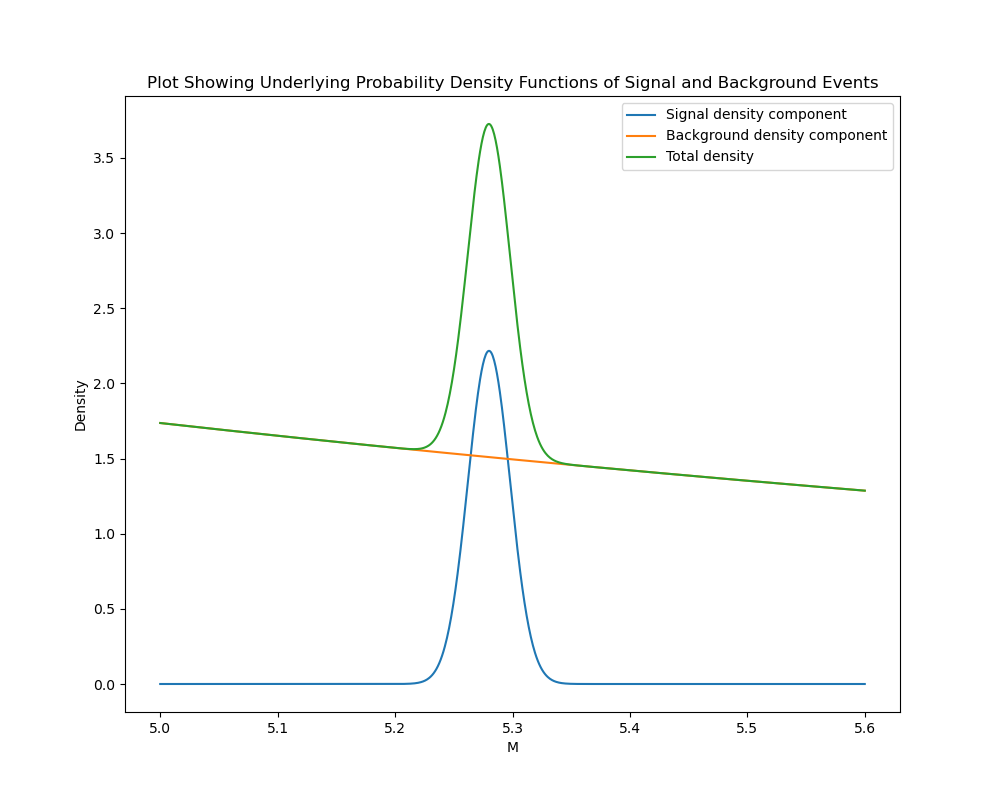
\includegraphics[scale=0.5]{part_d_plot.png}
    \caption{The true underlying distribution of $M$ [generated in Python using Matplotlib].}
    \label{partd}
\end{figure}

Note that the blue and orange lines, labelled as `density components' are the plots of the probability density functions for $M$ for the signal and background events respectively.
However, to make the plot more intuitive, they have been multiplied by the respective proportion of that type of event in the total population.
This means that technically neither is a probability density function, however their sum is the true mixed density for the population.
The area under either of the component functions limited to an interval smaller than $[5, 5.6]$ is precisely the probability that an event randomly sampled from the population will be of that kind, and lie within said interval.

\subsection*{Part (e)}

In part (e)

\begin{figure}[hbt]
    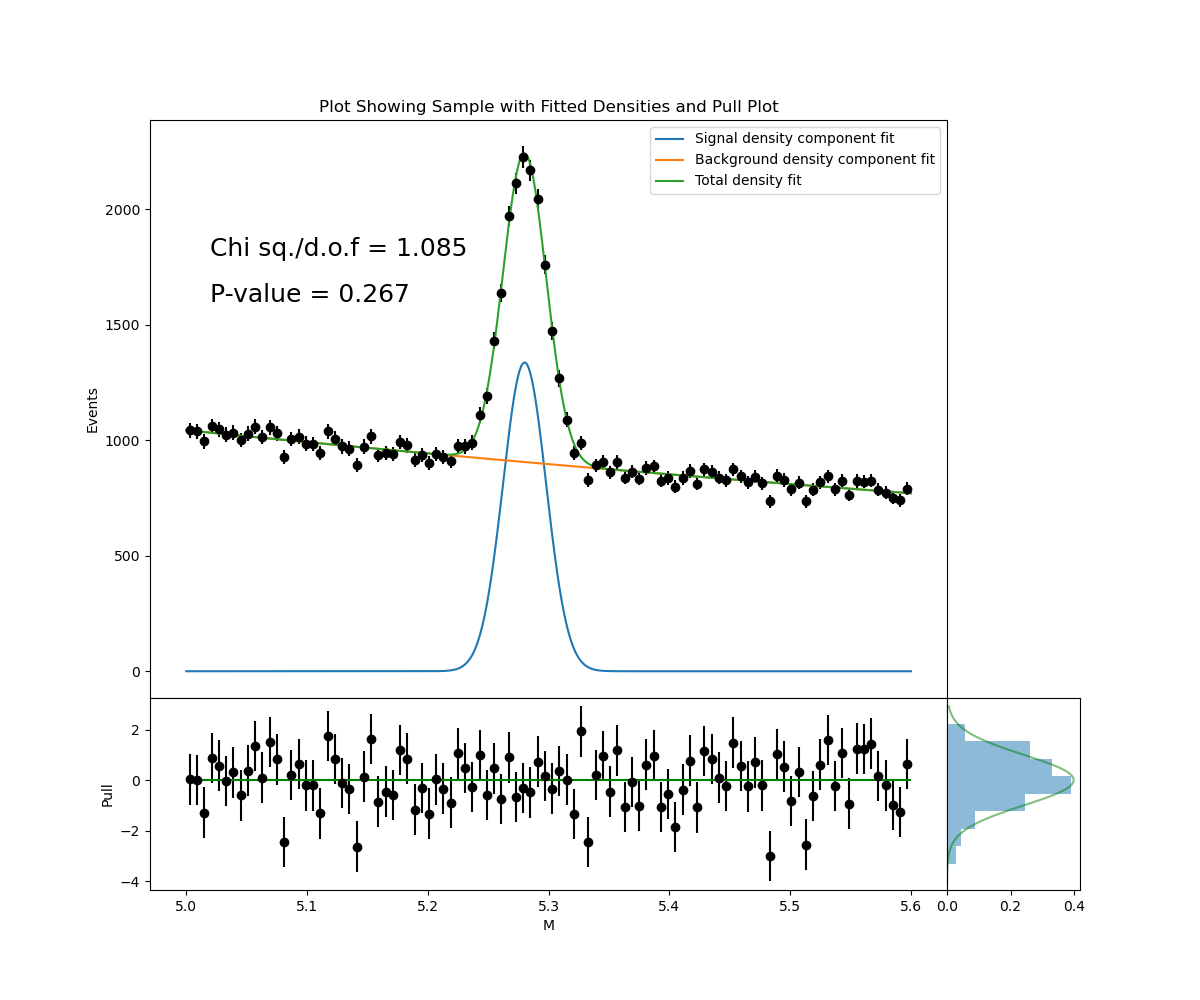
\includegraphics[scale=0.4]{part_e_plot.png}
    \caption{The true underlying distribution of $M$ [generated in Python using Matplotlib].}
    \label{parte}
\end{figure}

\section*{Section B}


\end{document}
